% ------------------------------------------------------------------------------
\section{Trabalhos Relacionados} \label{rel}
% TODO: Go back to here to customize this section.
% Currently it is to centered on ME optimization. 
% It does not mention interfaces, etc.

% + Related Work
% This section make an overview of the strategies to optimize the time performance of ME:
% algorithmic optimizations (fast-search algorithms, macroblock subsampling,
% sample truncation, multi-resolution ME, subsampled motion-field estimation),
%  parallelization of algorithms (our case), and
% hardware implementations of algorithms.
%
% Focus on works related to ME parallelization / distribution.
% Maybe compare to the work of Ronaldo's student: Ricardo Kintschner also about
% ME optimization on Cell (Webmedia2011).
% Look for other works directly comparable.
%
% Also: ?[and reviews techniques about designing for interfaces]?
% 

	Para a concepção deste trabalho foram consultados alguns trabalhos relacionados, dentre eles vale destacar o estudo e desenvolvimento realizado por Correll, Barendt e Branicky \cite{Correll}. Uma implementação {\it software-only}, chamada de PTPd. A sincronização de tempo com PTP se baseia na troca de mensagens que sincronização, que possuem um {\it timestamp} associado, entre o mestre e os escravos. Estes {\it timestamps} de alta precisão podem ser conseguidos com o auxílio de hardware especializado na camada física da rede, no entanto, não foi utilizado nenhum hardware especializado. Implementações {\it software-only} efetuam o {\it timestamp} em camadas mais altas da rede, o que acaba por introduzir graus de não-determinismo nas latências, conhecido como {\it jitter}. Alcançar a sincronização exata entre os dispositivos pertencentes à rede é o principal obstáculo no projeto de implementações deste tipo.
	
	O {\it daemon} foi desenvolvido para sistemas de Testes e Medições. Para tais sistemas o PTP proporciona sincronização de tempo e frequência. As necessidades destes sistemas influenciaram significativamente o resultado deste trabalho. Por ser uma implementação {\it software-only} ele não apresenta algumas funcionalidades encontradas em implementações assistidas por hardware. Realizar o registro do {\it timestamp} em camadas altas das camadas de protocolo, ao invés de realizar tal função próximo à camada física da rede. É utilizado um {\it software clock}, no entanto,  para os experimentos o sistema foi equipado com um relógio de hardware. Isso foi feito para permitir que o relógio pudesse ser lido com {\it jitter} mínimo.
	
	O PTPd se destina à sistemas embarcados que possuem recursos computacionais limitados. Isso inclui plataformas com sub-100MHz de CPU. Sendo assim o {\it daemon} utilizou cerca de $1\%$ da CPU de um processador de 66 MHz m68k. Além disso, o PTPd não requer uma unidade de ponto flutuante (FPU), ou emulação de FPU, pois utiliza somente aritmética de ponto fixo.
	
	Além do PTPd podemos citar outra grande implementação para sincronizar tempos de relógios largamente utilizado, o NTP, que segundo a definição de Minar o protocolo cria uma rede de hospedeiros na internet que sincronizam o tempo \cite{Minar1999}. A topologia do NTP pode ser vista na Figura 1. O NTP é construído sobre o {\it Internet Protocol} (IP), e no {\it User Datagram Protocol} ( UDP ), que provê um mecanismo de transporte sem a necessidade de estabelecer conexões entre os envolvidos \cite{Mills1994}. Este foi desenvolvido a partir do protocolo de tempo e da mensagem de {\it timestamp} {\it Internet Control Message Protocol} (ICMP), especialmente para manter a exatidão e a redundância.
		
	No modelo proposto para o NTP não houve nenhum esforço especial para realizar a descoberta de {\it peers}, configuração ou aquisição, apesar de haver implementações que contemplam estes aspectos. A integridade dos dados é proporcionada pelos {\it checksum's} do IP e do UDP, sendo que nenhum mecanismo de detecção de dados duplicados ou retransmissão são oferecidos. Dado o fato de apenas um formato de mensagem NTP ser utilizado, este protocolo é facilmente implementado e utilizado nos diversos sistemas operacionais existentes.
			
		\begin{figure}[ht]
		\begin{center}
		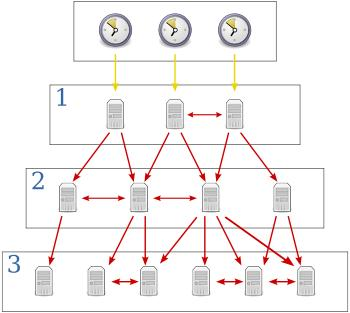
\includegraphics[scale=0.6, width=7cm]{fig/NTP1.jpg}
		\caption{Hierarquia no protocolo NTP}
		\end{center}
		\end{figure}
		
		O funcionamento do NTP consiste basicamente na troca de {\it timestamps} entre os servidores pertencentes a rede, estes {\it timestamps} são então utilizados para determinar os atrasos bidirecionais individuais, os {\it offsets} dos relógios e as estimativas de erros \cite{Mills1994}.
			
			
			\begin{figure}[ht]
				\begin{center}
				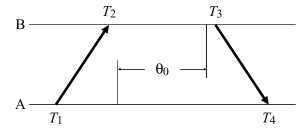
\includegraphics[scale=0.6, width=5cm]{fig/ntp3.jpg}
				\caption{{\it Timestamps} trocados pelo NTP \cite{Mills1994}}
				\end{center}
				\end{figure}
					
		De posse destas informações, há a necessidade de uma nova implementação do protocolo PTP, visto que o {\it daemon} proposto engloba a versão 1 do protocolo, enquanto que na versão 2 houveram melhorias, podendo citar a redução do tamanho da mensagem de sincronização, que facilita a sua implementação para sistemas embarcados. Além disso, o PTP permite obter um nível de precisão maior do que o obtido com o NTP \cite{DelRio2012}. 		
			
			
		%NTP timestamps are numbered and exchanged between peers A and B. Let T1, T2, T3, T4 be the values of the four most recent timestamps as shown and, without loss of generality, assume T3 > T2. Also, for the moment assume the clocks of A and B are stable and run at the same rate. Let
		%a = T2 − T1 and b = T3 − T4.
	%	If the network delay difference from A to B and from B to A, called differential delay, is small, % the clock offset θ and roundtrip delay δ of B relative to A at time T4 are close to
	%	θ = a + b 2
	%	and δ = a − b. (2)
	%	Each NTP message includes the latest three timestamps T1, T2 and T3, while the fourth T4 is determined upon arrival. Thus, both peers A and B can independently calculate delay and offset using a single bidirectional message stream. This is a symmetric, continuously sampled, time-transfer scheme similar to those used in some digital telephone networks
	%	B T2 T3
		
	% %	[LIN80]. Among its advantages are that errors due to missing or duplicated messages can be avoided.
	%	In [MIL92b] an exhaustive analysis is presented of the time and frequency errors that can accrue as the data are processed and refined at various levels in the subnet hierarchy. While the analysis is too long to repeat here, the results define the maximum error that can accrue under any operational condi- tion, called the synchronization distance λ, and the error expected under nominal operating conditions, called the dis- persion ε. There are several components of ε, including:
		%1. The maximum error in reading the local clock and each peer clock, which depends on the clock %resolution and method of adjustment.
		%2. The maximum error due to the frequency tolerance of the local clock and each peer clock since the time either was last set.
		%3. The estimated error contributed by each peer clock due to delay variations in the network and statistical latencies in the operating systems on the path to the primary reference source, which depends on differences between successive measurements for each peer clock. This is called the peer dispersion.
		%4. The estimated error contributed by the combined set of peers used to discipline the local clock, which depends upon the differences between individual members of the set. This is called the select dispersion.
	%	In practice, errors due to network delays usuually dominate ε. However, it is not possible to characterize these delays as a stationary random process, since network queues can grow and shrink in chaotic fashion and packet arrivals are fre- quently bursty. However, the method of calculating ε, as defined in the NTP Version 3 specification, represents a conservative estimate of the errors due to each of the above causes.
			
			
			
% ------------------------------------------------------------------------------
